\begin{figure}[htb]
  \centering
%segundo bloco de figuras
  \begin{tabular}{c c c c c }
    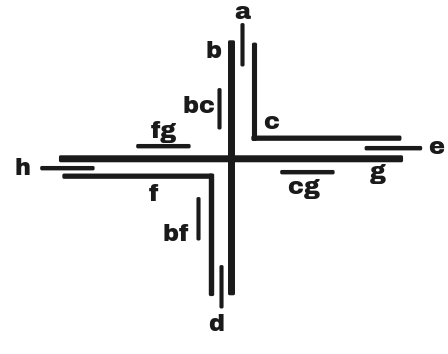
\includegraphics[width=4cm]{./img/falsePie.png}  %\label{fig:falsePie} 
    & &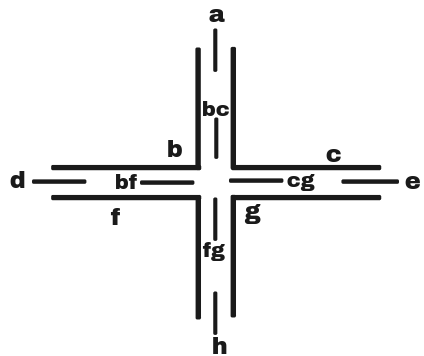
\includegraphics[width=4cm]{./img/truePie.png} %\label{fig:truePie}
    & &
 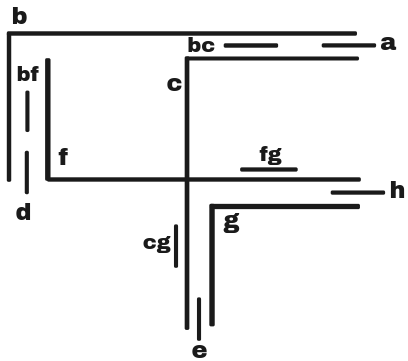
\includegraphics[width=4cm]{./img/frame.png} \\%[\abovecaptionskip]
    {\footnotesize (a) Baseada em false pie}  & &  {\footnotesize(b) Baseada em true pie} & & {\footnotesize (c) Baseada em frame} %\label{fig:frame}
  \end{tabular}
  \caption{Diferentes representações de dobra simples para o grafo  $H$ usando uma  false pie (a), uma true pie (b) e um frame (c) para representar o $C_4^{H}$}\label{fig:falsepietruepieframe}
\end{figure} 